%----------------------------------------------------------------------------
% 5. Beszámoló az implementáció folyamatáról
%   - Telepítés során meghozott (rossz) döntések
%   - (rossz) tapasztalatok
%
% A tervezés részletes leírása, a döntési lehetőségek értékelése és a
% választott megoldások indoklása

%\chapter{Introduction}
%\chapter{Earlier monitoring systems implemented in the dormitory}
%\chapter{Requirements of the new monitoring system}
%\chapter{Available industry standard technologies}
%\chapter{System architecture}
\chapter{Implementation details and experiences \label{ch5}}
%\chapter{Results and evaluation}
%\chapter{Future development opportunities}
%----------------------------------------------------------------------------

With the requirements and the system architecture defined we have a clear path
ahead ourselves. There are still quite a few decisions to be made and problems
to be solved. We are going to explore these in this chapter.

%----------------------------------------------------------------------------
\section{The server hardware and the host system}
%----------------------------------------------------------------------------

\subsection{The Hardware}

The hardware was inherited from previous monitoring projects. The machine is a
ProLiant DL360e Gen8 with two Intel Xeon E5-2450L CPUs, 32GBs of RAM, four
Gigabit Ethernet ports, 2x120GB SSDs and 2x1TB HDDs. This should be perfect to
serve our needs.

\subsection{The Operating System}

For the host operating system we are going to use a Linux distribution aimed at
servers. We have several choices here favouring ones that \kszk already
operate. These are: Ubuntu, Debian and Rocky Linux.

Ubuntu is developed and maintained by Canonical, a UK-based company. It had
been a popular choice among desktop and server Linux users alike. Unfortunately
it's most recent developments such as snaps made many previous users dislike
this system and migrate to others.

Debian is developed and maintained by a community of volunteers from around the
world. It is known for its stability and reliability, making it a popular
choice for servers and other mission-critical systems. It also has a large
repository of pre-compiled software packages, making it easy to install and
manage applications. Ubuntu is also based on Debian.

Rocky Linux is based on the codebase of Red Hat Enterprise Linux (RHEL), but is
developed and maintained by a community of volunteers. It aims to provide a
secure and stable platform that is compatible with RHEL, while also being free
of any vendor restrictions or licensing fees. It also comes with SELinux
preconfigured, making it more secure.

\subsection{The Kubernetes Distribution}

As for a Kubernetes distribution we of course have k8s. K8s supports everything
we need, however it is aimed at larger installations and multi-node clusters
thus it is harder to configure and more resource-intensive. A better
alternative is k3s, which is a lightweight, open-source Kubernetes distribution
that is designed to be easy to install and operate on resource-constrained
environments, such as edge computing or IoT devices. K3s also supports SELinux
and works perfectly with Rocky Linux.

\subsection{The Final Host System Configuration}

For the above reasons we decided to use Rocky Linux as the host OS, k3s as the
Kubernetes distribution and we are going to install VictoriaMetrics and Grafana
on top of these.

We installed the host system on the two SSDs configured as Linux Software RAID1
for redundancy and better uptime. The data is going to be stored on the two
HDDs for which we used ZFS and the HDDs are configured as a two-way mirror
(equivalent to a RAID1 in redundancy).

ZFS supports many advanced features besides different redundancy levels such as
encryption, checksumming, compression and snapshots. Although we do not yet
make use of these we have the opportunity to enable them in the future without
worrying about migration of the system which would couse unnecessary downtime.

Another issue we need to take care of is reproducibility. As setting up such a
system takes much time, effort and research it's not enough to only document
this progress. During migration to new hardware (in case of an upgrade or a
catastrophical failure) we would have to repeat all this work. To solve this we
chose to use Ansible which is already widely used by \kszk.

Ansible is an open-source IT automation tool that allows users to configure and
manage systems, deploy applications, and automate processes. It uses YAML files
just like the rest of our tools, and then uses a series of modules to enforce
that state on the system.

Every change is going to be applied through Ansible and every file used is
going to be stored on a repository on \kszk's GitLab server.

%----------------------------------------------------------------------------
\section{Preparing the k3s Kubernetes distribution}
%----------------------------------------------------------------------------

On it's own, Kubernetes is a very powerful tool. It can handle many containers,
services, load balancers and much more. But even a single pod contains at least
one docker container. It's configuration is managed via YAML files but this way
of management becomes repetitive very quickly (imagine repeating the same port
numbers over many configuration files) violating the DRY (Don't Repeat
Yourself) principle and becomes a nightmare to maintain. To overcome this issue
the community had created several tools to ease it's use.

\subsection{Management Tools}

The k3s kubernetes distribution can be managed the same way as it's
heavywheight, full-fledged k8s brother. Thus we are going to use the same tools
we'd use on a more complicated deployment.

Managing a kubernetes cluster can be (and I usually done) remotely. By this I
don't mean an SSH session - the Kubernetes command-line tool, \verb+kubectl+
tool runs on any administrator's machine and for authentication we need to copy
the \verb+/etc/rancher/k3s/k3s.yaml+ configuration file from the k3s host
machine.

Now we have the power to manage our cluster yet this does not free us from
writing complicated, thousands-of-lines long YAML configuration files for
deployment. The solution is Helm.

Helm is an open-source package manager for Kubernetes that allows users to
easily install, upgrade, and manage applications on Kubernetes clusters. Helm
uses a packaging format called charts, which are pre-configured templates that
define the desired state of an application, including its dependencies,
configuration, and resources.

\subsection{Persistent Volumes}

VictoriaMetrics' and Loki's stateful components are going to need a persistent
volume which we want to store on our ZFS mirror. Persistent volumes are going
to be provided by the OpenEBS ZFS CSI Driver. Installation is easy:
\verb+kubectl apply -f https://openebs.github.io/charts/zfs-operator.yaml+.

We have to configure the driver to use our pool.

\begin{lstlisting}[language=yaml,caption=zfs-localpv.sc.yaml]
apiVersion: storage.k8s.io/v1
kind: StorageClass
metadata:
  name: openebs-zfspv
parameters:
  recordsize: "4k"
  compression: "off"
  dedup: "off"
  fstype: "zfs"
  poolname: "spinningrust/openebs-zfspv"
provisioner: zfs.csi.openebs.io
\end{lstlisting}

Configuration is applied yet again by the following command:
\verb+kubectl apply -f zfs-localpv.sc.yaml+.

% install krew for kubectl
% install minio for kubectl

%----------------------------------------------------------------------------
\section{Installing and configuring a basic VictoriaMetrics on k3s}
%----------------------------------------------------------------------------

Now that we have set up k3s we can begin installing and configuring
VictoriaMetrics.

Before we continue let's take a look at how Helm works. Complex, multi-pod
kubernetes systems are set up by many large YAML files. These files contain
redundant informations, hard to comprehend and difficult to work with. Helm
uses template files (which use Go syntax) which handle everything that can be
computed, and so called values files. The latter contain sane default
configurations where such things make sense and require the user to enter
values where no such configurations can exist, for example external services'
authentication details. The combination of these is called a helm chart. Helm
charts can be added to the system manually or by adding a helm chart
repository.

\subsection{Downloading the Helm Charts}

First of all we are going to add the VM helm chart repository following the
intructions on VM's GitHub repository:
\url{https://github.com/VictoriaMetrics/helm-charts}.

\begin{lstlisting}
helm repo add vm https://victoriametrics.github.io/helm-charts/
helm repo update
\end{lstlisting}

Next, we are going to select the helm chart that fits our needs. The repository
contains many charts most of which only contain a subset of a full
VictoriaMetrics stack. The one we need is \verb+victoria-metrics-k8s-stack+,
this is the full k8s VM stack.

Before installing this we have to configure it through the correct values file.
We can get the values file with the help of the \verb+helm show values+
command:

\begin{lstlisting}
helm show values vm/victoria-metrics-k8s-stack > values.yaml
\end{lstlisting}

For the initial \verb+values.yml+ see Appendix~\ref{vmValues}.

\subsection{Installing VictoriaMetrics}

Once the \verb+values.yml+ is configured the helm chart is installed with the
following command:

\begin{lstlisting}
helm install beholder vm/victoria-metrics-k8s-stack -f values.yml
\end{lstlisting}

%----------------------------------------------------------------------------
\section{Collecting metrics}
%----------------------------------------------------------------------------

With VictoriaMetrics up and running we can begin collecting our metrics from
various servers and network devices. In fact, we are already collecting some
metrics: the helm chart used before already configured the monitoring of
VictoriaMetrics, k3s and the host node itself.

The stack installed also contains another powerful feature: the VictoriaMetrics
Kubernetes Operator.

An operator is a piece of software that extends the Kubernetes API to create,
configure, and manage instances of complex applications. This allows you to use
the Kubernetes API to automate tasks such as deploying, scaling, and backing up
your applications. They provide a declarative way to describe the desired state
of an application, and then automatically reconciling the actual state of the
application with the desired state.

\subsection{Collecting Metrics from Servers}

We are going to add 3 servers for demontration purposes:
\begin{itemize}
	\item memory-alpha and memory-beta: this is a ZFS-based storage server cluster
	\item trash: this server provides music for \kszk's hard-working members
\end{itemize}

To collect metrics from a remote system the target host must have the
neccessary exporters installed and configured. Exporters are a piece of
software that collect metrics from system components and expose them throug an
HTTP API. Different kinds of exporters collect different metrics: the generic
node exporter collect basic statistics such as CPU and RAM usage, while
specialized exporters are needed to collect metrics from components such as
ZFS, mailing servers or databases.

After the desired exporters are installed and configured on the target host we
have to inform VictoriaMetrics about their existence. For this we have to
define \verb+VMStaticScrape+ objects, apply these configurations and let the
operator configure the \verb+vmagnet+ component to collect metrics from these
servers as well. The configuration is as follows:

\begin{lstlisting}[language=yaml,caption=Configuration file for memory-alpha and memory-beta]
apiVersion: operator.victoriametrics.com/v1beta1
kind: VMStaticScrape
metadata:
  name: memory-alpha-and-beta
  namespace: monitoring
spec:
  targetEndpoints:
    - targets:
        - 10.0.69.101:9100
        - 10.0.69.102:9100
  jobName: memory-alpha-and-beta
\end{lstlisting}

\begin{lstlisting}[language=yaml,caption=Configuration file for trash]
apiVersion: operator.victoriametrics.com/v1beta1
kind: VMStaticScrape
metadata:
  name: trash
  namespace: monitoring
spec:
  targetEndpoints:
    - targets:
        - 152.66.209.79:9100
  jobName: trash
\end{lstlisting}

The \verb+.metadata.name+ and \verb+.metadata.namespace+ values identify the
resouce, while key-value pairs under the \verb+.spec+ key define the
configuration itself. The \verb+.spec.targetEndpoints.targets+ array contain
the ip+port pairs for every available exporter, while \verb+.spec.jobName+ is
used to locate the collected metrics inside \verb+vmagent+ and \verb+Grafana+.

These files contain many boilerplate around little information. Luckily we have
a solution for this which we going to explore in the next section.

The monitoring server has a dedicated interface in the administration VLAN just
like every other server operated by \kszk - this means that we can reach these
targets directly.

\subsection{Collecting Metrics from Network Devices}

Monitoring network devices is slightly more complicated.  Network devices can
not run arbitrary softwares such as exporters and these devices can only be
reached on a physically separated network knowns as the management LAN. Luckily
we can reach the NOCs (Network Operation Centers) which are connected to this
network. For the other part we must use some kind of exporter that runs
separately and collects data through SNMP.

The Prometheus project has a solution exactly for this:
\url{https://github.com/prometheus/snmp_exporter/tree/main/generator} and \kszk
already has an SNMP exporter with the required MIBs built in. We installed one
instance of this exporter on each NOC. The exporters are reached through a k3s
loadbalancer, this makes sure that the metrics are not duplicated and so far at
least one exporter is running metrics are going to be collected.

\begin{lstlisting}[language=yaml,caption=Load balancer configuration]
apiVersion: v1
kind: Service
metadata:
  name: noc-snmp-exporter
spec:
  ports:
    - port: 80
      targetPort: 9116
      name: exporter
      protocol: TCP
  type: ClusterIP

---
apiVersion: v1
kind: Endpoints
metadata:
  name: noc-snmp-exporter
subsets:
  - ports:
      - port: 9116
        name: exporter
        protocol: TCP
    addresses:
      - ip: 10.0.208.241
      - ip: 10.0.208.242
\end{lstlisting}

With all these set up we can scrape network devices just like we did with
servers. Below is showed the initial configuration scraping the core router
\verb+rtr-1+ only.

\begin{lstlisting}[language=yaml,caption=Initial SNMP scraping configuration]
apiVersion: operator.victoriametrics.com/v1beta1
kind: VMStaticScrape
metadata:
  name: schnet-snmp
  namespace: monitoring
spec:
  jobName: schnet-snmp
  targetEndpoints:
    - targets:
        - noc-snmp-exporter:80
      path: /snmp
      params:
        target: [ rtr-1 ]
        module: [ sch_core_net_mibs ]
\end{lstlisting}

Note that all network device metrics are reached through a single exporter. The
\verb+.spec.targetEndpoints.params.target+ key identifies the device.

\subsection{Metric Visualizations}

As for visualization, our \verb+Grafana+ comes with some common dashboards
preinstalled such as a node exporter, kubernetes exporter and VictoriaMetrics
dashboards. Other, commonly used dashboards can easily be imported from
\url{https://grafana.com/grafana/dashboards/}. Unique dashboards, such as the
ones displaying our SNMP metrics must be created by us.

\begin{figure}[!h]
	\centering
	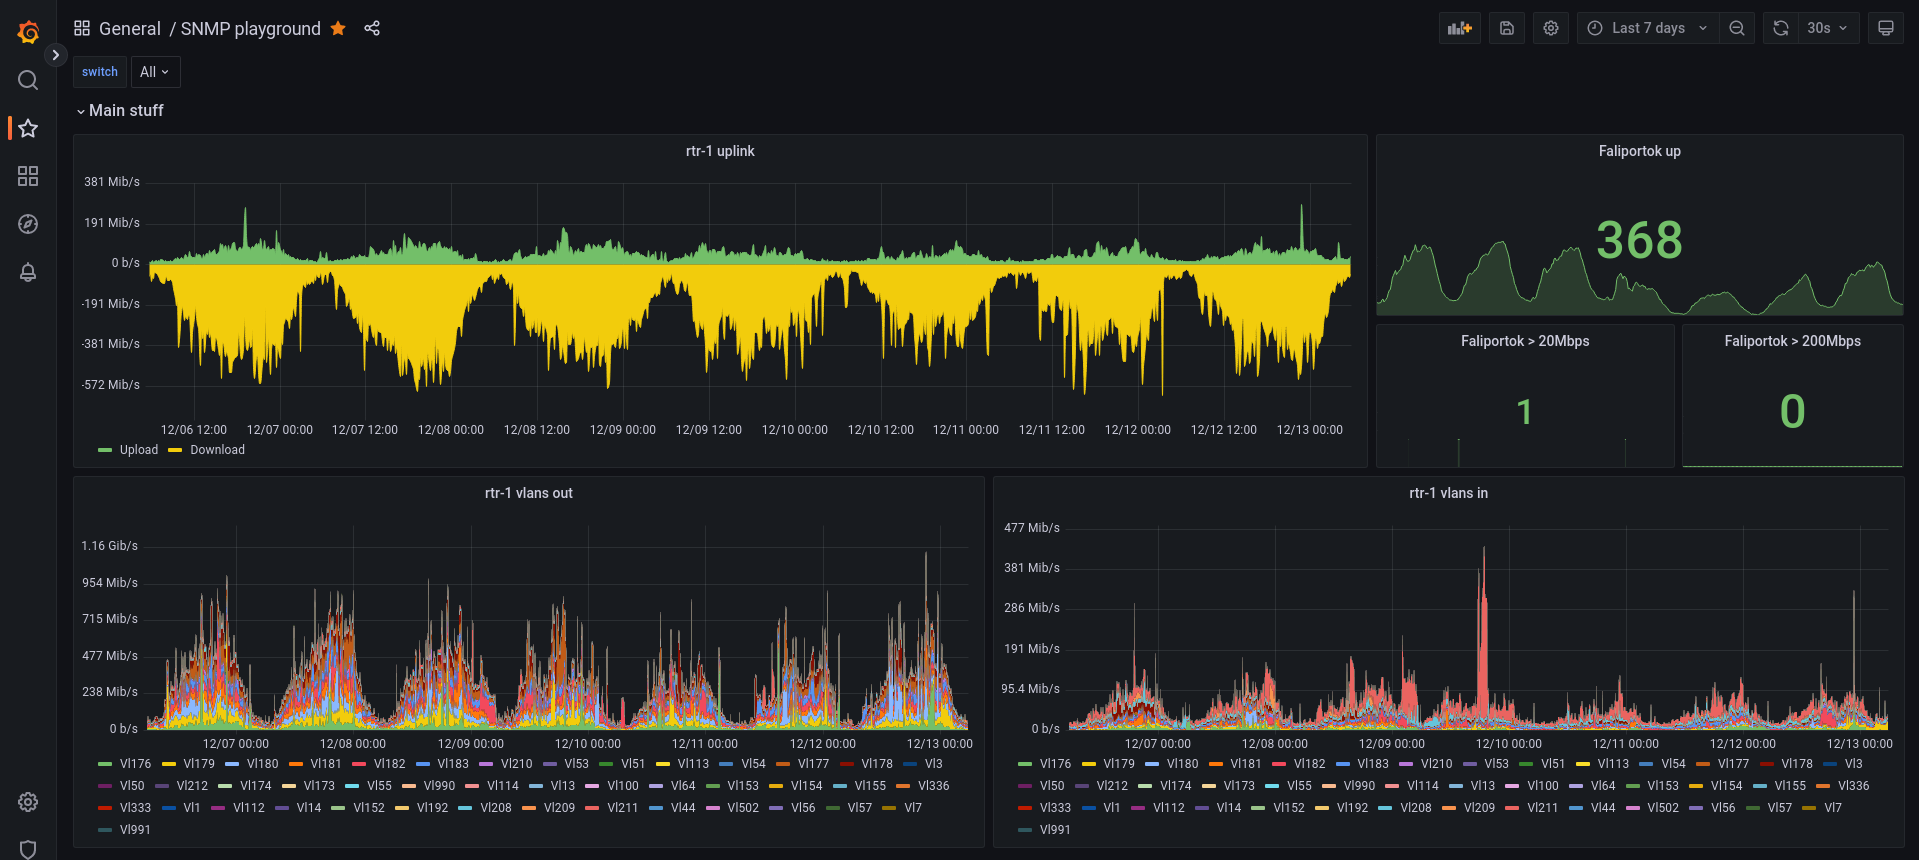
\includegraphics[width=150mm, keepaspectratio]{figures/grafana-snmp-playground.png}
	\caption{Screenshot of the Grafana SNMP Playground Dashboard at the time of writing}
\end{figure}

The above is shown a screenshot of the SNMP Playground dashboard. After the
initial version was released members of \kszk took their time and added many
other useful metrics to this visualization. The 'Faliportok up' panel shows
every active 1Gbit endpoint on the \sch's network. It shows nicely the least
actively used periods of the week: between 4am and 8am especially on the
weekends.

%----------------------------------------------------------------------------
\section{Automating tasks with the help of GitLab CI}
%----------------------------------------------------------------------------

Now we are able to monitor our servers and network devices. However as seen
above, configuration is very repetitive. Moreover, adding or modifiny any
device requires the contribution of the monitoring system administrator which
slows down the integration and wastes time that could be utilized better
elsewhere.

We already have a perfect tool for generating configurations: helm charts. We
can quickly and easily create simple ones ourselves. For defining a helm chart
we need:

\begin{itemize}
	\item \verb+./Chart.yaml+: this contains some required metadata about the chart itself
	\item \verb+./template/*.yaml+: these are the Go templates themselves, the final config will be generated from these files
	\item \verb+./template/*.tmpl+: these are helper template functions
	\item \verb+./values.yaml+: the values for the template
\end{itemize}

\subsection{Implementing Helm Charts for Configuration Generation}

Let's review the implementation of the node exporter helm chart.

\begin{lstlisting}[language=yaml,caption=./Chart.yaml]
apiVersion: v2
name: node-exporter-target
description: Scrape configs for Prometheus node exporter
type: application
version: 0.0.0
appVersion: "kolbaasz"
\end{lstlisting}

\begin{lstlisting}[language=yaml,caption=./templates/\_helpers.tmpl]
{{- define "name" }}
{{- .Chart.Name }}-{{.Release.Name}}
{{- end }}
\end{lstlisting}

\begin{lstlisting}[language=yaml,caption=./templates/node-exporter.yaml]
{{- $global := . }}
{{- range .Values.Devices }}
---
apiVersion: operator.victoriametrics.com/v1beta1
kind: VMStaticScrape
metadata:
  name: "{{ template "name" $global }}-{{ .Name }}"
  namespace: monitoring
spec:
  targetEndpoints:
    - targets:
        {{- range .Targets }}
        - "{{ . }}"
        {{- end }}
  jobName: "{{ .Name }}"
{{- end }}
\end{lstlisting}

\begin{lstlisting}[language=yaml,caption=./values.yaml]
Devices:
  - Name: memory-alpha-and-beta
    Targets:
      - 10.0.69.101:9100
      - 10.0.69.102:9100

  - Name: trash
    Targets: [ 152.66.209.79:9100 ]
\end{lstlisting}


These Go templates operate with the values file in context as \verb+.Values+.
This chart iterates over the \verb+.Values.Devices+ array's elements with the
\verb+range+ function, creates a \verb+VMStaticScrape+ object for each one.
Each \verb+VMWStaticScrape+'s \verb+.spec.targetEndpoints.targets+ array is
filled with the matching \verb+.Values.Devices.Targets+ array's elements.

Now when adding a new device the administrator only has to edit the
\verb+values.yml+ file which now only contains the neccessary informations
without any noise.

To start using this new method, first we have to install the helm chart:
\verb+helm install -n monitoring node-exporter-targets .+. For subsequent uses
we can upgrade the chart: \verb+helm upgrade -n monitoring node-exporter-targets .+.

We can generate SNMP monitoring configurations the same way. See the helm chart
in Appendix~\ref{snmpScraperChart}.

\subsection{Configuring GitLab CI}

We had achieved a way to write monitoring configurations easily but this
approach still requires the intervention of a precious sysadmin. Countionous
integration is our way to go. Our repository on \kszk's GitLab contains
everything needed to add new hosts to the system, let's make use of GitLab's
Contionous Integration (CI) features. For this the following
\verb+.gitlab-ci.yml+ file is going to be used.

\begin{lstlisting}[language=yaml,caption=.gitlab-ci.yml]
stages: [ sanity_check, upgrade_charts ]

before_script:
  - apk add diffutils
  - kubectl config use-context kszk/ansible/playbooks/monitoring:beholder

node_check:
  stage: sanity_check
  image: alpine/k8s:1.24.8
  script:
    - ./helmdiff.sh node-exporter-targets ./files/helm-charts/node-exporter-target
  only:
    changes:
      - files/helm-charts/node-exporter-target/**
      - .gitlab-ci.yml
      - helmdiff.sh

snmp_check:
  stage: sanity_check
  image: alpine/k8s:1.24.8
  script:
    - ./helmdiff.sh snmp ./files/helm-charts/snmp-exporter-target
  only:
    changes:
      - files/helm-charts/snmp-exporter-target/**
      - .gitlab-ci.yml
      - helmdiff.sh

node_export:
  stage: upgrade_charts
  image: alpine/k8s:1.24.8
  script:
    - helm upgrade -n monitoring node-exporter-targets ./files/helm-charts/node-exporter-target
  only:
    changes:
      - files/helm-charts/node-exporter-target/**
      - .gitlab-ci.yml
      - helmdiff.sh
    refs:
      - main

snmp_export:
  stage: upgrade_charts
  image: alpine/k8s:1.24.8
  script:
    - helm upgrade -n monitoring snmp ./files/helm-charts/snmp-exporter-target
  only:
    changes:
      - files/helm-charts/snmp-exporter-target/**
      - .gitlab-ci.yml
      - helmdiff.sh
    refs:
      - main
\end{lstlisting}

Note the \verb+helmdiff.sh+ script used above. We tried to use the already
available helm diff plugin but ran into several problems, the version we used
did not accept our new and completely valid configurations. For this reason we
used the following script:

\begin{lstlisting}[language=bash,caption=helmdiff.sh]
#!/bin/sh

set -ueo pipefail

release="$1"
chart="$2"

helm get manifest -n monitoring "$release" > /tmp/installed
helm template -n monitoring "$release" "$chart" > /tmp/new

diff -w --color=always -y /tmp/installed /tmp/new || [ "$?" = "1" ]
\end{lstlisting}

The CI scripts run on the monitoring server in docker inside an Alpine image.
The image is complemented with the \verb+diffutils+ package which is required
by the \verb+helmdiff.sh+ script. The CI runs on two stages for each of our
helm charts. The first stage, \verb+sanity_check+ verifies the syntactic
validity of our new configuration as well as displays the difference between
the current and the newly generated difference using \verb+helmdiff.sh+. On the
main branch the \verb+upgrade_charts+ stage upgrades our helm charts using the
new configurations. One job per helm chart is used in each stage and each job
is only ran when neccessary (i.e. when a change was made).

Using these tools new systems can be monitored with minimal knowledge and
without the intervention of a monitoring system administrator.

%----------------------------------------------------------------------------
\section{Authentication and authorization}
%----------------------------------------------------------------------------

So far our users can set up monitoring for any of their devices but we are far
from done. As only the hardcoded \verb+Administrator+ account can log into the
otherwise publicly available Grafana users can not make use of the system.

We are going to authenticate and authorize our users through AuthSCH with OAuth
2.0. Luckily Grafana supports this protocol. Unlucky for us Grafana expects the
user's e-mail to be at the \verb+/email+ path exactly and we found no way to
reconfigure this. For legacy reasons AuthSCH serves the e-mail in a different
path.

To work around this issue we created a very simple proxy server that translates
AuthSCH's response to the format expected by Grafana. Since the implementation
of this service is trivial we are not going to explore this further.

\begin{lstlisting}[language=yaml,caption=Grafana OAuth 2.0 configuration]
grafana:
  grafana.ini:
    auth.generic_oauth: # client is at Garmine's SCHAcc
      name: "AuthSCH"
      enabled: "true"
      client_id: "18023005984133885935"
	  client_secret: "secret" # Redacted for security purposes
      scopes: "basic displayName admembership linkedAccounts"
      auth_url: "https://auth.sch.bme.hu/site/login"
      token_url: "https://auth.sch.bme.hu/oauth2/token"
      api_url: "http://authsch-api-authsch.authsch-hack.svc/grafana" # ha-ha
      allow_sign_up: "true"
      role_attribute_path: "contains(adgroups[*], 'KSZK') && 'Admin' || contains(adgroups[*], 'KSZKUjonc') && 'Viewer' || 'Vesztettem'"
      role_attribute_strict: "true"
      groups_attribute_path: "adgroups"
\end{lstlisting}

The above is a pretty standard OAuth 2.0 configuration. Notable are the
different \verb+api_url+ path (these requests are routed through our proxy) and
the \verb+role_attribute_path+ value. The latter describes the authorization
based on AD group memberships. Members of the \verb+KSZK+ group are granted
\verb+Admin+ role: they are authorized to do make any changes in Grafana save
for a few things such as managing users and changing permissions. Members of
the \verb+KSZKUjonc+ group are granted \verb+Viewer+ role: they are authorized
to view almost any part of our Grafana but can not make any changes. Other
users would get \verb+Vesztettem+ which is a nonexsistent role, thus they are
denied logging in.

Superadmin rights are granted locally either through the above mentioned
\verb+Administrator+ account or by another superadmin account.

%----------------------------------------------------------------------------
\section{Collecting logs}
%----------------------------------------------------------------------------

\subsection{Configuring and Installing Loki}

We are going to use Loki for writing, storing and querying logs. Loki just like
VictoriaMetrics can be split into smaller services and installed in a larger,
distributed and scalable form as a cluster for heavier workloads. For smaller
infrastructures Loki can be installed as a single service as well which is
easier to configure and should fit our needs perfectly. For this we are going
to write Loki's \verb+loki-values.yml+ file.

First of all we are going to install the helm chart as before:

\begin{lstlisting}[language=bash,caption=Installing Loki's helm chart]
helm repo add grafana https://grafana.github.io/helm-charts
helm repo update
\end{lstlisting}

\begin{lstlisting}[language=yaml,caption=loki-values.yml]
loki:
  commonConfig:
    replication_factor: 1
  storage:
    type: filesystem
  server:
    log_level: warn

monitoring:
  selfMonitoring:
    enabled: false

test:
  enabled: false

write:
  replicas: 0

read:
  replicas: 0

singleBinary:
  replicas: 1
  persistence:
    size: 256Gi
    storageClass: openebs-zfspv

ingress:
  enabled: false

gateway:
  enabled: false

networkPolicy:
  enabled: false

minio:
  enabled: false
\end{lstlisting}

In order to configure Loki as a single binary we need a single replica of
\verb+singleBinary+ and no \verb+write+ and \verb+read+ replicas. Logs are
going to be stored on a persistent volume provided by \verb+openebs-zfspv+. For
now we are going to disable selfmonitoring and testing as well.

Once the configuration is ready we are going to install as usual:
\verb+helm install --values loki-values.yaml loki grafana/loki+

Loki only receives logs from another service and does no processing on them. In
order to send logs to Loki we are going to use Promtail. Promtail is very
versatile, is able to receive and collect logs from various sources and can
process the logs before sending them. We are going to split the responsibility
of collecting and processing logs. Logs are going to be collected and sent by
the hosts themselves either via Promtail (for servers) or syslog (for more
simple devices such as routers and switches). Processing the logs is going to
be done by a Promtail instance running on the monitoring system. This way
target hosts can send logs with minimal and very simple configurations while
the monitoring system administrators can configure log processing locally,
without having access to the target hosts.

\subsection{Collecting Logs of the Monitoring System}

The first target for log collecting is the monitoring system itself. So far
only the system administrators had access to these logs via the
\verb+kubectl logs+ command. Having access to these logs would make debugging
much easier for our users.

\begin{lstlisting}[language=yaml,caption=local-promtail-values.yml]
daemonset:
  enabled: false

deployment:
  enabled: true
  replicaCount: 1

serviceMonitor:
  enabled: true

config:
  logLevel: warn
  serverPort: 3101
  clients:
    - url: http://loki:3100/loki/api/v1/push
  snippets:
    common:
      - action: replace
        target_label: job
        replacement: beholder-pods
\end{lstlisting}

The local Promtail's configuration is changed minimally: since we are running a
single node kubernetes cluster we opt for a single replica deployment,
\verb+serviceMonitor+ is enabled for the VictoriaMetrics operator and collected
logs' are stored under the `beholder-pods` job for easy identification.

\subsection{Receiving and Processing Logs from other Systems}

The other Promtail instance is going to receive, process and then send the
remotely collected logs to Loki. Let's take a look at it's configuration.

\begin{lstlisting}[language=yaml,caption=promtail-values.yml]
daemonset:
  enabled: false

deployment:
  enabled: true
  replicaCount: 1

defaultVolumes: []
defaultVolumeMounts: []

serviceMonitor:
  enabled: true

extraPorts:
  syslog:
    name: tcp-syslog
    containerPort: 1514
    protocol: TCP
    externalTrafficPolicy: Local
    service:
      type: ClusterIP # TODO make LoadBalancer after auth has been figured out
      port: 1514
  promhttp:
    name: prom-http
    containerPort: 3500
    protocol: TCP
    service:
      type: ClusterIP
      port: 3500
  promgrpc:
    name: prom-grpc
    containerPort: 3600
    protocol: TCP
    service:
      type: ClusterIP
      port: 3600

config:
  file: |
    server:
      log_level: info
      http_listen_port: 3101
    clients:
      - url: http://loki:3100/loki/api/v1/push

    positions:
      filename: /run/promtail/positions.yaml

    scrape_configs:
      - job_name: syslog
        syslog:
          listen_address: 0.0.0.0:1514
          labels:
            job: syslog
        relabel_configs:
          - source_labels: [ __syslog_message_hostname ]
            target_label: host
          - source_labels: [ __syslog_message_severity ]
            target_label: severity
          - source_labels: [ __syslog_message_facility ]
            target_label: facility
          - source_labels: [ __syslog_message_app_name ]
            target_label: app
            
      - job_name: prom
        loki_push_api:
          server:
            http_listen_port: 3500
            grpc_listen_port: 3600
          labels:
            job: prom

    limits_config: {}
\end{lstlisting}

Similarly to the local Promtail we opt for a single replica deployment. As we
do not with to collect local logs with this instance we disable
\verb+defaultVolumes+ and \verb+defaultVolumeMounts+. The \verb+extraPorts+ map
configures Promtail to accept connections from syslog and other Promtail
instances. The \verb+config.file+ is just a string, literally the contents of
Promtail's configuration file. The above is just a simple forwarding for
Promtail and syslog, with added label translation for syslog.

Installation is done with \verb+helm install+ for both charts just as before.

For demonstration purposes we installed a Promtail instance on a server called
\verb+trash+. After setting up a Grafana dashboard we are able to successfully
browse \verb+trash+'s logs.

\newpage

\subsection{Log Visualization}

\begin{figure}[!h]
	\centering
	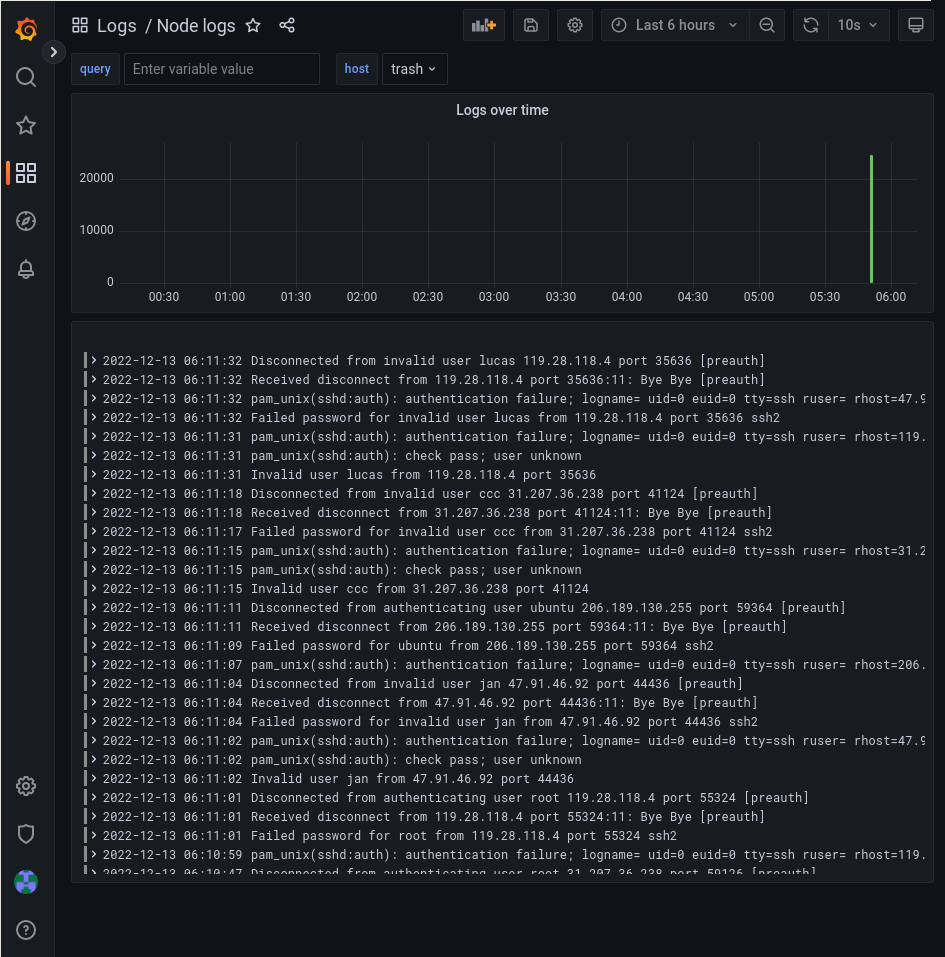
\includegraphics[width=150mm, keepaspectratio]{figures/grafana-logs-trash.png}
	\caption{Screenshot of the Grafana Logs dashboard just after implementation}
\end{figure}

Above is seen a screenshot of the Grafana Logs dashboard. On the logs collected
from Trash, \kszk's media-player VM we can see several unsuccessful log-in
attempts from various botnets.

\subsection{Security}

For security purposes authentication is mandatory for receiving logs. Both
Promtail->Promtail and syslog->Promtail ways are able to use authentication. As
many network devices don't support anything else than sending logs via
unauthenticated and unencrypted syslog we have postponed this feature.

%----------------------------------------------------------------------------
\section{Creating alerts and sending notifications}
%----------------------------------------------------------------------------

In the monitoring stack the \verb+vmalert+ component communicates with the
VictoriaMetrics TSDB, has access to every metric and executes recording and
alerting rules. Recording rules' results are written back to the TSDB while
alerting rules send notifications to the \verb+vmalertmanager+ component. The
alert manager then routes these alerts to various receivers. Receivers then
finally format and send out alerts to external platforms. These include but are
not limited to: e-mail, Slack API, Telegram and HTTP.

\subsection{Configuring VMAlert}

Our \verb+vmalert+ configuration is very plain. The bulk of it's configuration,
the alerting and recording rules are applied through the VictoriaMetrics
kubernetes operator.

\begin{lstlisting}[language=yaml,caption=vmalert configuration]
vmalert:
  annotations: {}
  enabled: true
  spec:
    selectAllByDefault: true
    image:
      tag: v1.83.0
    evaluationInterval: 15s

  templateFiles:
    {}

  ingress:
    enabled: false
\end{lstlisting}

Luckily the kubernetes VictoriaMetrics stack comes with a plethora of alerting
rules preconfigured. Some of these alerts only fire on VictoriaMetrics' error
conditions while others are applied for every monitored node such as NTP out of
sync and RAID error alerts.

\begin{lstlisting}[language=yaml,caption=Example alerting rule configuration]
apiVersion: operator.victoriametrics.com/v1beta1
kind: VMRule
metadata:
  name: beholder-victoria-metrics-k8s-stack-node-exporter
  namespace: monitoring
spec:
  groups:
  - name: node-exporter
    rules:
    - alert: NodeClockSkewDetected
      annotations:
        description: Clock is out of sync by more than 300s. Ensure NTP is configured correctly on this host.
        runbook_url: https://runbooks.prometheus-operator.dev/runbooks/node/nodeclockskewdetected
        summary: Clock skew detected.
      expr: |-
        ( node_timex_offset_seconds >  0.05 and deriv(node_timex_offset_seconds[5m]) >= 0 )
        or
        ( node_timex_offset_seconds < -0.05 and deriv(node_timex_offset_seconds[5m]) <= 0 )
      for: 10m
      labels:
        severity: warning
\end{lstlisting}

The above is an example for alerting when the system clock drifts more than 300
seconds on any monitored node.

\subsection{Configuring VMAlertmanager}

These alerting rules are ideal for demonstration purposes and are also useful
for real-life scenarios. But with nowhere to go they would be worthless, so
let's configure our alert manager to send everything to \kszk's Mattermost
server's \verb+~alerts-test+ channel for now.

\begin{lstlisting}[language=yaml,caption=alertmanager configuration]
alertmanager:
  enabled: true
  spec:
    selectAllByDefault: true
    externalURL: ""
    routePrefix: /

  config:
    global:
      resolve_timeout: 5m
	  slack_api_url: "https://127.0.0.1" # Redacted for security reasons

    templates:
      - "/etc/vm/configs/**/*.tmpl"
    route:
      group_by: ["alertgroup", "job"]
      group_wait: 30s
      group_interval: 5m
      repeat_interval: 12h
      receiver: "mattermost"

    receivers:
      - name: "mattermost"
        slack_configs:
          - channel: "#alerts-test"
            username: "SCP-049"
            send_resolved: true
            title: '{{ template "slack.monzo.title" . }}'
            icon_emoji: '{{ template "slack.monzo.icon_emoji" . }}'
            color: '{{ template "slack.monzo.color" . }}'
            text: '{{ template "slack.monzo.text" . }}'
            actions:
              - type: button
                text: "Runbook :green_book:"
                url: "{{ (index .Alerts 0).Annotations.runbook_url }}"
              - type: button
                text: "Dashboard :grafana:"
                url: "{{ (index .Alerts 0).Annotations.dashboard }}"
              - type: button
                text: "Silence :no_bell:"
                url: '{{ template "__alert_silence_link" . }}'

  # better alert templates for slack
  # source https://gist.github.com/milesbxf/e2744fc90e9c41b47aa47925f8ff6512
  monzoTemplate:
    enabled: true

  templateFiles:
    {}

  ingress:
    enabled: false
\end{lstlisting}

Mattermost uses the Slack API for incoming webhooks. This sample
\verb+alertmanager+ config uses trivial routing. A single failure usually
triggers more alerts at once so it only tries to send alerts as a batch in a
single message instead of one-by-one in order to reduce noise. The receiver
config on the other hand hilights some nice features:

\begin{itemize}
	\item we receive a notification when the cause is fixed
	\item the monzo templates nicely decorate the message
	\item we get a button to the relevant runbook (basically a manual for the alert)
	\item we get a button to the relevant Grafana Dashboard
	\item we get a button that silences the alert
\end{itemize}

\newpage

\subsection{Alerts on Mattermost}

After applying the new configuration using \verb+helm upgrade+ we instantly
receive several alerts on Mattermost's \verb+~alerts-test+ channel that had
been stuck in the queue.

\begin{figure}[!h]
	\centering
	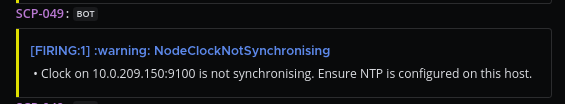
\includegraphics[width=150mm, keepaspectratio]{figures/mattermost-alert-x-ray.png}
	\caption{Screenshot of a real alert on \kszk's Mattermost server}
\end{figure}

Above is shown a real alert sent from VictoriaMetrics to \kszk's Mattermost
server. This alert unexpectedly unveiled a real problem: one of our servers
system clock did not properly synchronise via NTP. The difference was around
500 milliseconds.

As it turns out the Mattermost API is not 100\% compatible with Slack's: even
though both support interactive messages and buttons we do not get them with
the alert messages.

\subsection{Implementing Continous Integration for Alerts}

Even though the preconfigured alerts are useful we want to give out users the
ability to define their own alerts. For this we are going to use GitLab CI as
well.

Ideally we would have a single helm chart for everything: monitoring, logging
and alerting configurations. This would eliminate every repetition and with a
preconfigured rules library would make alerting much more simple. This would
require lots of work and careful planning. This is out of the scope for this
project and thus we have opted for a much more trivial solution. See the helm
chart for adding alerting and recording rules in
Appendix~\ref{snmpScraperChart}.

We installed the helm chart usnig the \verb+helm install+ command and added the
following new jobs to \verb+.gitlab-ci.yml+

\begin{lstlisting}[language=yaml,caption=New jobs in .gitlab-ci.yml]
alerts_check:
  stage: sanity_check
  image: alpine/k8s:1.24.8
  script:
    - ./helmdiff.sh kszk-alerts ./files/helm-charts/kszk-alerts
  only:
    changes:
      - files/helm-charts/kszk-alerts/**
      - .gitlab-ci.yml
      - helmdiff.sh

alerts_upgrade:
  stage: upgrade_charts
  image: alpine/k8s:1.24.8
  script:
    - helm upgrade -n monitoring kszk-alerts ./files/helm-charts/kszk-alerts
  only:
    changes:
      - files/helm-charts/kszk-alerts/**
      - .gitlab-ci.yml
      - helmdiff.sh
    refs:
      - main
\end{lstlisting}

Although it's more complicated than ideal we gave our users the tools
neccessary to configure their own alerting and recording rules without the
intervention of a monitoring system administrator.
